\documentclass{article}
\usepackage{amsmath, booktabs,comment, graphicx, subcaption}

\begin{document}

\title{self-adaptative genetic algorithm for minimum thickness laminated composite design}
In this study, an self-adaptative genetic algorithm(SAGA) is proposed to minimize thickness(or weight) of
laminated composite subject to in-plane loading. Fiber orientation angles and ply thickness are
chosen as design variables. By imposing safety factor as the constraint, SAGA is used to search the optimal design of a laminated composite under
virous loading cases. To check the feasibility of a laminated lay-up, Tsai-wu failure criterion is
taken to calculate the safety factor.



\section{Introduction}
thickness\cite { schmit1973optimum, schmit1977optimum, fukunaga1991strength, soares1995discrete,
	le1995improved, jayatheertha1996application, wang1996optimum, adali1997minimum,
	correia1997higher, scares1997optimization, abu1998optimum, lombardi1998anti, le1998design,
	sivakumar1998optimum, barakat1999use, richard2000reliability, moita2000sensitivity,
soremekun2001composite, walker2003technique, di2003multiconstrained, kere2003using}

In practice, fiber orientations are restricted to a finite set of angles, and layer thickness is
a specific numberic value. 

\section{Analysis of }

\subsection{Stress and Strain in a Lamina}
For a single lamina has a small thickness under plane stress, and it's upper and lower surfaces of the lamina are
free from external loads. According to the Hooke's Law, the three-dimensional stress-strain equations can be reduced to
two-dimensional stress-strain equations. The stress-strain relation in local axis 1-2 is:
\begin{equation}
    \begin{bmatrix}
        \sigma _1\\
        \sigma _2\\
        \tau_{12}
    \end{bmatrix}
    =
    \begin{bmatrix}
        Q_{11} & Q_{12} & 0\\
        Q_{12} & Q_{22} & 0\\
        0      &  0     & Q_{66}
    \end{bmatrix}
    \begin{bmatrix}
        \varepsilon_1\\
        \varepsilon_2\\\gamma_{12}
    \end{bmatrix}
\end{equation}
where $Q_{ij} $are the stiffnesses of the lamina that are related

to engineering elastic constants given by
\begin{equation}
    \begin{split}
    &Q_{11}=\frac{E_1}{1-v_{12}v_{21}}\\
    &Q_{22}=\frac{E_2}{1-v_{12}v_{21}}\\
    &Q_{66}=G_{12}\\
    &Q_{12}=\frac{v_{21}E_2}{1-v_{12}v_{21}}\\
    \end{split}
\end{equation}

where $E_1, E_2, v_{12}, G_{12} $ are four independent engineering elastic constants, which are defined as follows: $E_1 $ is the longitudinal Young's modulus, $E_2 $ is the transverse Young's modulus, $v_{12} $ is the major Poisson's ratio, and $G_{12} $ is the in-plane shear modulus.

Stress strain relation in the global x-y axis:
\begin{equation}\left[\begin{array}{l}\sigma _{x} \\ \sigma _{y} \\ \tau_{xy}\end{array}\right]=\left[\begin{array}{lll}\bar{Q}_{11} & \bar{Q}_{12} & \bar{Q}_{16}\\ \bar{Q}_{12} & \bar{Q}_{22} & \bar{Q}_{26} \\ \bar{Q}_{16} & \bar{Q}_{26} &\bar{Q}_{66}\end{array}\right]\left[\begin{array}{l}\varepsilon_{x} \\ \varepsilon_{y}\\ \gamma_{x y}\end{array}\right]
\end{equation}
where

\begin{equation}
	\begin{array}{l}
		\resizebox{.35\textwidth}{!}{$\bar{Q}_{11}=Q_{11} c^{4}+Q_{22} s^{4}+2\left(Q_{12}+2
		Q_{66}\right) s^{2} c^{2}$} \\

		\resizebox{.35\textwidth}{!}{$\bar{Q}_{12}=\left(Q_{11}+Q_{22}-4 Q_{66}\right) s^{2}
		c^{2}+Q_{12}\left(c^{4}+s^{2}\right)$} \\

		\resizebox{.35\textwidth}{!}{$\bar{Q}_{22}=Q_{11} s^{4}+Q_{22} c^{4}+2\left(Q_{12}+2
		Q_{66}\right) s^{2} c^{2}$} \\

		\resizebox{.4\textwidth}{!}{$\bar{Q}_{16}=\left(Q_{11}-Q_{12}-2 Q_{66}\right) c^{3} s-\left(Q_{22}-Q_{12}-2Q_{66}\right) s^{3} c$}
		 \\ 
		\resizebox{.4\textwidth}{!}{$\bar{Q}_{26}=\left(Q_{11}-Q_{12}-2 Q_{66}\right) c s^{3}-\left(Q_{22}-Q_{12}-2 Q_{66}\right)c^{3} s$}
		 \\ 
	\resizebox{.4\textwidth}{!}	{$\bar{Q}_{66}=\left(Q_{11}+Q_{22}-2 Q_{12}-2 Q_{66}\right)
	s^{2}c^{2}+Q_{66}\left(s^{4}+c^{4}\right)$}\\
	\end{array}
\end{equation}


The c and s denotes $cos\theta $ and $sin\theta $.

The local and global stresses in an angle lamina are related

to each other through the angle of the lamina $\theta $
\begin{equation}\left[\begin{array}{l}\sigma _{1} \\ \sigma _{2} \\ \tau_{12}\end{array}\right]=[T]\left[\begin{array}{l}\sigma _{x} \\ \sigma _{y} \\\tau_{xy}\end{array}\right]
\end{equation}

where
\begin{equation}[T]=\left[\begin{array}{ccc}c^{2} & s^{2} & 2 s c \\ s^{2} & c^{2} & -2 s c \\ -s c & s c &c^{2}-s^{2}\end{array}\right] 
\end{equation}



\subsection{Stress and Strain in a Laminate}
\begin{equation} \label{eq:force_and_moments}
	\begin{array}{l}
		\begin{aligned}
	\begin{bmatrix}
		N_x \\
		N_y \\
		N_{xy}
	\end{bmatrix}
	&=
	\begin{bmatrix}
		A_{11} & A_{12} & A_{16} \\
		A_{12} & A_{22} & A_{26} \\
		A_{16} & A_{26} & A_{66} 
	\end{bmatrix}
    \begin{bmatrix}
		\varepsilon_x^0 \\
        \varepsilon_y^0 \\
		\gamma_{xy}^0
    \end{bmatrix}   \\
	&+               
	\begin{bmatrix}
		B_{11} & B_{12} & B_{16} \\
		B_{11} & B_{12} & B_{16} \\
		B_{16} & B_{26} & B_{66} 
	\end{bmatrix}
	\begin{bmatrix}
		k_x \\
		k_y \\
		k_{xy} 
	\end{bmatrix}  \\
\end{aligned} \\ \\
\begin{aligned}
	\begin{bmatrix}
		M_x \\
		M_y \\
		M_{xy}
	\end{bmatrix}
	&=
	\begin{bmatrix}
		B_{11} & B_{12} & B_{16} \\
		B_{12} & B_{22} & B_{26} \\
		B_{16} & B_{26} & B_{66} 
	\end{bmatrix}
    \begin{bmatrix}
		\varepsilon_x^0 \\
        \varepsilon_y^0 \\
		\gamma_{xy}^0
    \end{bmatrix} \\ 
	&+  
	\begin{bmatrix}
		D_{11} & D_{12} & D_{16} \\
		D_{11} & D_{12} & D_{16} \\
		D_{16} & D_{26} & D_{66} 
	\end{bmatrix}
	\begin{bmatrix}
		k_x \\
		k_y \\
		k_{xy} 
	\end{bmatrix}
\end{aligned}
	\end{array}
\end{equation}


$N_x,N_y $  - normal force per unit length

$N_{xy} $  - shear force per unit length

$M_x, M_y $ - bending moment per unit length

$M_{xy} $  - twisting moments per unit length

$\varepsilon^{0}, k $- mid plane strains and curvature of a laminate in x-y coordinates

The mid plane strain and curvature is given by
\begin{equation}
    \begin{split}
    &A_{ij}=\sum_{k=1}^{n}(\overline{Q_{ij}})_k(h_k-h_{k-1})  i=1,2,6, j=1,2,6\\
    &B_{ij}=\frac{1}{2}\sum_{k=1}^{n}(\overline{Q_{ij}})_k(h_k^2 - h_{k-1}^2)  i=1,2,6, j=1,2,6\\
    &D_{ij}=\frac{1}{3}\sum_{k=1}^{n}(\overline{Q_{ij}})_k(h_k^3 - h_{k-1}^3) i=1,2,6, j=1,2,6\\
    \end{split}
\end{equation}

The [A], [B], and [D] matrices are called the extensional, coupling, and bending stiffness matrices,
respectively. The extensional stiffness matrix $[A]$ relates the resultant in-plane forces to the
in-plain strains, and the bending stiffness matrix $[D]$ couples the resultant bending moments to
the plane curvatures.  The coupling stiffness matrix $[B]$ relates the force and moment terms to the
midplain strains and midplane curvatures.


\section{Failure Theory for a lamina}
Many different theories about the failure of an angle lamina have been developed for a
unidirectional lamina, such as the maximum stress failure theory, maximum strain failure theory,
Tsai-Hill failure theory, and Tsai-Wu failure theory. The failure theories of a lamina are based on
the stresses in the local axes in the material. There are four normal strength parameters and one shear
stress for a unidirectional lamina. The five strength parameters are:

$(\sigma _1^{T})_{ult}= $ ultimate longitudinal tensile strength

$(\sigma _1^{C})_{ult}= $ ultimate longitudinal compressive strength

$(\sigma _2^{T})_{ult}= $ ultimate transverse tensile strength

$(\sigma _2^{C})_{ult}= $ ultimate transverse compressive strength 

$(\tau_{12})_{ult}= $ and ultimate in-plane shear strength

In the present study, Tsai-wu failure theory is taken to decide whether a lamina fails,
because this theory is more general than the Tsai-Hill failure theory, which considers two
different situations, the compression and tensile strengths of a lamina. A lamina is considered to fail
if \begin{equation} \label{eq:tsai_wu}
\begin{split}
	H_1 \sigma_1  & + H_2 \sigma_2 + H_6 \tau_{12} + H_{11}\sigma_1^2 + H_{22} \sigma_2^2 \\
				  & + H_{66}  \tau_{12}^2 + 2H_{12}\sigma_1\sigma_2 < 1
\end{split}
\end{equation}

is violated, where

\begin{equation} \label{eq:sr}S R=\frac{\text {Maximum Load Which Can Be Applied}}{\text {Load Applied}}
\end{equation}


\subsection{Failure Theories for a Laminate}
If keep increasing the loading applied to a laminate, the laminate will fails. The failure process
of a laminate is more complicate than a lamina, because a laminate consists of multiple plies, and
the fiber orientation, material, thickness of each ply maybe different from the others. In most
situations, some layer fails first and the remains continue to take more loads until all the plies
fail.  If one ply fails, it means this lamina does not contribute to the load carrying capacity of
the laminate. The procedure for finding the first failure ply given follows the fully discounted
method:

\begin{enumerate}
\item Compute the reduced stiffness matrix [Q] referred to as the local axis for each ply using its four engineering elastic constants $E_1 $, $E_2 $, $E_{12} $, and $G_{12} $.

\item Calculate the transformed reduced stiffness $[\bar{Q}] $ referring to the global coordinate system (x, y) using the reduced stiffness matrix [Q] obtained in step 1 and the ply angle for each layer.

\item  Given the thickness and location of each layer, the three laminate stiffness matrices [A], [B], and [D] are determined.

\item  Apply the forces and moments, $[N]_{xy}, [M]_{xy} $ solve
Equation \ref{eq:force_and_moments}, and calculate the middle plane strain $[\sigma ^{0}]_{xy} $ and curvature $[k]_{xy} $.

\item Determine the local strain and stress of each layer under the applied load.

\item  Use the ply-by-ply stresses and strains in the Tsai-wu failure theory to find the strength
	ratio, and the layer with smallest strenght ratio is the first failed ply. 
\end{enumerate}




\section{Methodology}
\subsection{Objective function}
There are two design variables here, the angles in the laminate, and the number of layers that each
fiber orientation has. The objective function is as

$F  = 2t_0 \sum_{k=1}^n n_k$ 

The first term represent the total thickness of the composite laminates, $t_0$ is ply thickness;
$n_k$ is the number of plies in the kth lamina, in which the fiber orientation is $\theta_k$.

The only constraint is the safety factor of the material under certain loading, and it should
greater than 1.

\subsection{Selection}
The purpose of the selection operator is how to chose parents to produce children of better
fitness. Traditional methods of selecting strategies only take the fitness of the individual into
acount, however, becasue of the existance of constraint, the selection strategies have to change a
little bit. The parents of next generation consists of three groups: proper groups, active groups,
and potential groups. 

Proper parents mean individual fullfils the constraint, which are chosen by the individual's
fitnees, individuals with better fitness are more likely to be chosen if they fit the constraint;
active groups means that individual is supposed to be always exist in the parents during the GA,
which are selected by fitness, ignoring the constraint; potential groups means that they are likely
to turn into proper individual after a couple of generations, and potential individuals are chosen
by constraint function, the more the individual fulfils the constraint, the more possiblity it will
be selected.


	
\subsection{Crossover}
The crossover operator happens among these three groups. the child of two proper groups are more
likely to be a proper individual which can be used to obtain a better individual. the child of an
active individual and a potential individual can significantly change the gene of active
individual's chromsome, which lets the individual evolved toward a new direction.  The offspring of
two active individuals are more likely to be an active individual, which can maitain the active
group.
\subsection{Mutation}
A mutation direction is imposed on the mutation operator which to make sure the individual evolving
toward the right direction. The mutation direction, denoted by $md$, is a n dimensional vector corresonding to
number of constraints, it is decided by the constraint thresholds $CT_i$ and the current individual's
constraint value, denoted as $CV_i$,  The mutation vector can be obtained by the following formula

$\text{md} = [CT_1, \cdots, CT_{n-1}, CT_n] -  [CV_0, \cdots, CV_{n-1}, CV_n]$

During the operator, the mutation consists of three parts, the length of the chromsome, the angle
of the chromsome, and the number of each angle. Becasue the chromsome's length is positive correlated with the individual's
fitness, the coefficient of length mutation denoted by $C_l$, if $\sum_{i=1}^{N}{CT_i}$ great than
zero, the mutation length is restricted to the range $[0,C_l \sum_{i=1}^{N}{CT_i}]$; if the
$\sum_{i=1}^{N}{CT_i}$ less than zero, the mutation length is restricted to the range
$[0,\sum_{i=1}^{N}{CT_i}]$; Assuming a $[13_6/-27_4]_s$ carbon T300/5308 composite laminate under
the loading $N_{xx} = N_{yy} = 10$ MPa m, the only constraint is the safety factor greater than 1.
Accoring to the Tsai-Wu criterion, its safety factor is 0.0539. So the mutation vector is $[0.941]$,
assuming the coefficient is 20, so the mutation range is from 0 to 18. A random number is generated
from the range $[0, 18]$, supposing the outcome is 13, then a length generator is used to a list,
the it's sum is 13, suppose the list is [5, 8], the laminate after mutation is $[13_{11}/-27_{12}]_s$.


The relationship between the angles in the composite laminate and the chromsome's fitness is
unclear, so the mutation direction of chromsome's angle is random. The coefficient angle mutation is
$C_a$, $[0,C_a \sum_{i=1}^{N}{CT_i}]$


\section{Result}
In this experiment, only one constraint is imposed on the composite laminates which is the safety
factor $CT_1$, and its value is 1. The constraint value of individual is $CV_1$. So the mutation
vector here is a one dimensional vector $[1 - CV_1 ]$, and the coefficient of length mutation $C_l$ and
angle mutation $C_a$, respectively, chosen here is 20 and 10. 

\begin{figure}[!t]
	\centering
		\begin{subfigure}[b]{0.8\linewidth}
			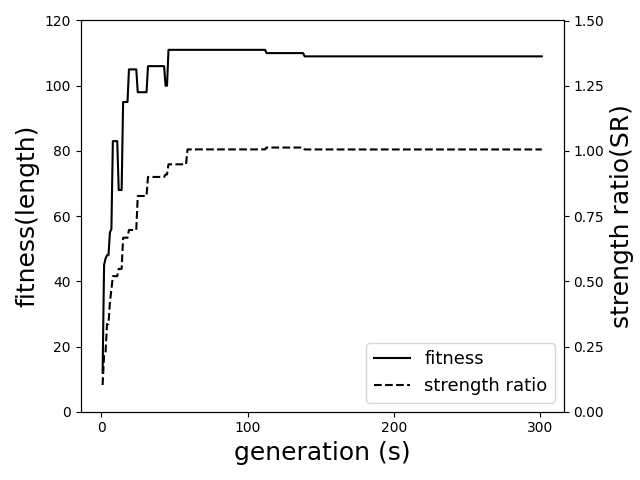
\includegraphics[width=\linewidth]{2020-11-10-pre-image/two_distinct_angle_fitness_and_sr.png}
		\end{subfigure}

		\begin{subfigure}[b]{0.8\linewidth}
			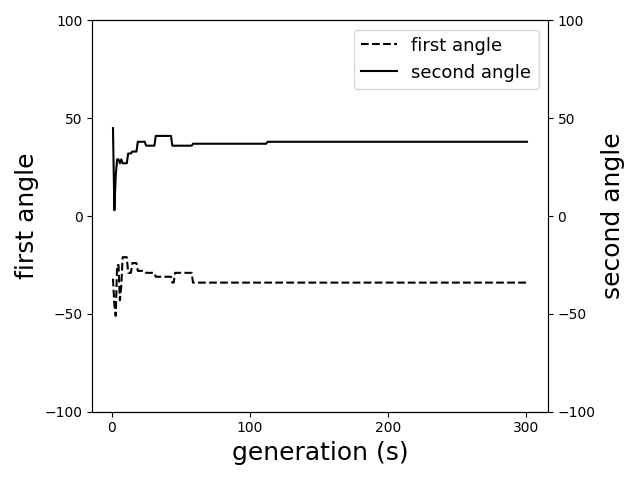
\includegraphics[width=\linewidth]{2020-11-10-pre-image/two_distinct_angle_angle_change.png}
		\end{subfigure}

		\begin{subfigure}[b]{0.8\linewidth}
			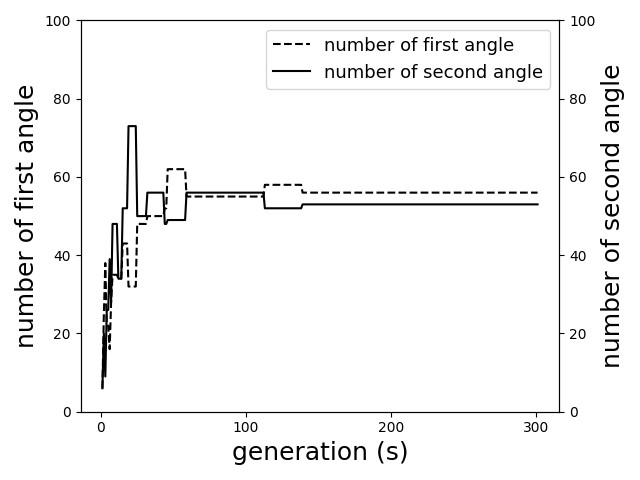
\includegraphics[width=\linewidth]{2020-11-10-pre-image/two_distinct_angler_number_change.png}
		\end{subfigure}
	\caption{Two distinct angles}
	\label{fig:two_angles}
\end{figure}



Figure \ref{fig:two_angles} (a) shows how the optimal individual's fitness and strength
ratio vary during the GA process. The method to chose optimal individual considering two following
situations, if no individual in the current population meets constraint, the one with biggest
fitness is selected as the optimal individual; if there are one or multiple individuals fullfils
requirement, the one with smallest fitness is chosen.  Figure \ref{fig:two_angles} (b) shows how the two distinct fiber
orientation changes at the same time, and Figure  \ref{fig:two_angles} (c) how the number of each angles change.

	At the beginning of this GA process, the fitness curves increased very quickly, becasue of
individual's strength ratio $CT_0$ is very small, so the difference between the individual's fitness and
the imposed constraint threshold is a big positive number, so the range of mutaion length is from 0
to $C_l(CT_0 - CV_0)$. The length of individual increases by n, which is random number between 0 and 
$C_l(CT_0 - CV_0)$. As can be seen from Figure \ref{fig:two_angles} (a), both of optimal
individual's fitness and strength ratio increases very quickly.  The range of mutaion angle is from
0 to $C_a(CT_0 - CV_0)$, and the number of every angle also change violently. During this stage,
increasing individual's length playing a major role in increasing individual's fitness.

After a couple of generations, the optimal individual's fitness get bigger, and the difference
between individual's fitness and constraint threshold get smaller. The range of mutaion length $[0,
C_l(CT_0 - CV_0)]$ turn smaller. At this stage, simply increase the individual's length doesn't make
much difference in improve individual's fitnees, and a better composite laminates lay-up can
dramaticly change the optimal individual's fitness. That's why the fitness curve oscillated
violently in this stage.  At the same time, the strength ratio curve kept growing smoothly. But the
growing speed got more smaller.

When GA comes to its last phase, GA found individuals that meet the constraint. Now the optimal
individual's fitness is greater than the safety factor. The range of mutation length is from 
$C_l(CT_0 - CV_0)$ to 0. It means individuals need to decrease it's length and improve its internal
structure to meet the constraint. That's why the fitness of optimal individual kept decreaing,
however, the strength ratio curve still is greater then safety factor.

\begin{figure}[!t]
	\centering
		\begin{subfigure}[b]{0.8\linewidth}
			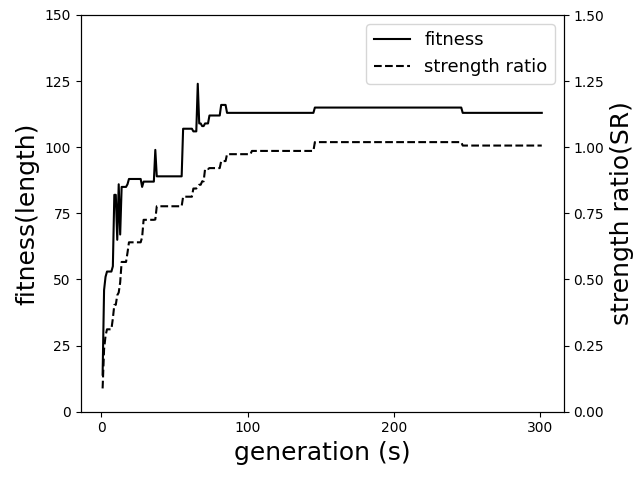
\includegraphics[width=\linewidth]{2020-11-10-pre-image/Three_distinct_angles_fitness_and_sr.png}
		\end{subfigure}

		\begin{subfigure}[b]{0.8\linewidth}
			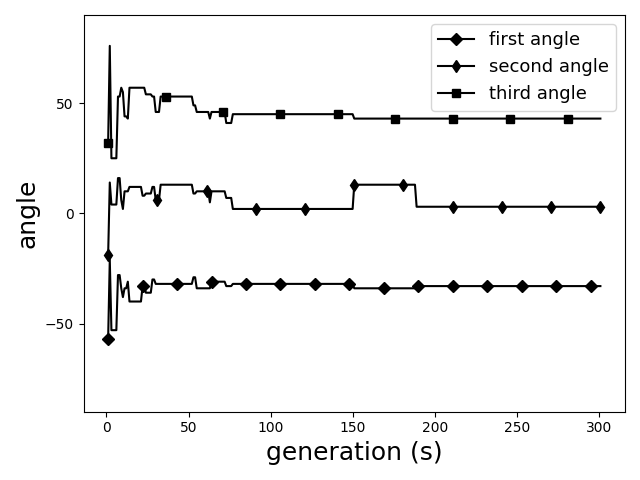
\includegraphics[width=\linewidth]{2020-11-10-pre-image/three_distinct_angles_angle_change.png}
		\end{subfigure}

		\begin{subfigure}[b]{0.8\linewidth}
			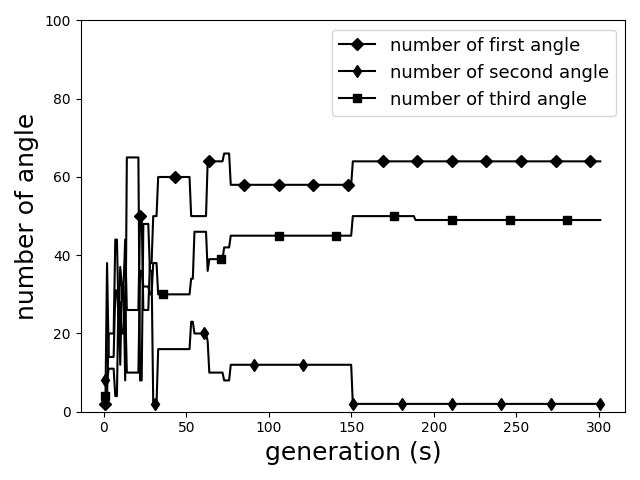
\includegraphics[width=\linewidth]{2020-11-10-pre-image/three_distinct_angle_number_of_angle.png}
		\end{subfigure}
	\caption{Three distinct angles}
	\label{fig:three_angles}
\end{figure}



\begin{table*}
%% increase table row spacing, adjust to taste
%\renewcommand{\arraystretch}{1.3}
% if using array.sty, it might be a good idea to tweak the value of
% \extrarowheight as needed to properly center the text within the cells
\caption{An Example of a Table}
\label{T300/5308 material properties}
\centering
%% Some packages, such as MDW tools, offer better commands for making tables
%% than the plain LaTeX2e tabular which is used here.
\begin{tabular}{cccc}
	\toprule
	Property								   & Symbol				  & Unit  &  Graphite/Epoxy     \\
	\midrule
	Longitudinal elastic modulus			   & $E_1$				  & GPa   &  181                 \\
	Traverse elastic modulus				   & $E_2$				  & GPa   &  10.3                \\
	Major Poisson's ratio					   & $v_{12}$			  &       &  0.28                \\
	Shear modulus							   & $G_{12}$			  & GPa   &  7.17                \\
	Ultimate longitudinal tensile strength     & $(\sigma_1^T)_{ult}$ & MP    &  1500                 \\
	Ultimate longitudinal compressive strength & $(\sigma_1^C)_{ult}$ & MP    &  1500                 \\
	Ultimate transverse tensile strength       & $(\sigma_2^T)_{ult}$ & MPa   &  40                   \\
	Ultimate transverse compressive strength   & $(\sigma_2^C)_{ult}$ & MPa   &  246                   \\
	Ultimate in-plane shear strength           & $(\tau_{12})_{ult}$  & MPa   &  68                    \\
	Density                                    & $\rho$               & $g/cm^3$ &  1.590                    \\
	\bottomrule
\end{tabular}
\end{table*}


% Note that IEEE does not put floats in the very first column - or typically
% anywhere on the first page for that matter. Also, in-text middle ("here")
% positioning is not used. Most IEEE journals/conferences use top floats
% exclusively. Note that, LaTeX2e, unlike IEEE journals/conferences, places
% footnotes above bottom floats. This can be corrected via the \fnbelowfloat
% command of the stfloats package.


\begin{table*}
%% increase table row spacing, adjust to taste
%\renewcommand{\arraystretch}{1.3}
% if using array.sty, it might be a good idea to tweak the value of
% \extrarowheight as needed to properly center the text within the cells
\caption{The optimum lay-ups using two distinct fiber angles under various biaxial loading cases}
\label{tab:two_distinct_angle}
\centering
%% Some packages, such as MDW tools, offer better commands for making tables
%% than the plain LaTeX2e tabular which is used here.
\begin{tabular}{cccc}
	\toprule
	Loading	$N_{x}/N_{y}/N_{xy}$ (MPa m)	       & Optimum lay-up sequences                                   & laminate thickness &  Safety factor \\
	\midrule
	10/5/0                                         &  $[33_{29}/\text{-}39_{25}/\bar{\text{-}39}]_s$            &     109               &  1.0074 \\
	20/5/0                                         &  $[33_{22}/\text{-}31_{24}]_s$                             &     92               &  1.0055 \\
	40/5/0                                         &  $[29_{18}/\text{-}21_{23}/\bar{\text{-}23}]_s$            &     83               &  1.0034 \\
	80/5/0                                         &  $[\text{-}20_{27}/21_{25}/\bar{25}]_s$                    &     105               &  1.0029 \\
	120/5/0                                         &  $[\text{-}18_{34}/17_{36}]_s$                            &     140               &  1.0000 \\
	\bottomrule
\end{tabular}
\end{table*}

\begin{table*}
%% increase table row spacing, adjust to taste
%\renewcommand{\arraystretch}{1.3}
% if using array.sty, it might be a good idea to tweak the value of
% \extrarowheight as needed to properly center the text within the cells
\caption{The optimum lay-ups using three distinct fiber angles under various biaxial loading cases}
\label{T300/5308 material properties}
\centering
%% Some packages, such as MDW tools, offer better commands for making tables
%% than the plain LaTeX2e tabular which is used here.
\begin{tabular}{cccc}
	\toprule
	Loading	$N_{x}/N_{y}/N_{xy}$ (MPa m)	       & Optimum lay-up sequences                                   & laminate thickness &  Safety factor \\
	\midrule
	10/5/0                                         &  $[37_{27}/\text{-}38_{27}/\text{-}5]_s$                   &     110               &  1.0023 \\
	20/5/0                                         &  $[34_{24}/\text{-}32_{14}/\text{-}28_{11}]_s$             &     98               &  1.0237 \\
	40/5/0                                         &  $[21_{28}/\text{-}32_{19}/2_3]_s$                         &     100               &  1.0788 \\
	80/5/0                                         &  $[\text{-}21_{25}/\text{-}16_{3}/21_{26}]_s$              &     108               &  1.0128 \\
	120/5/0                                         &  $[\text{-}18_{34}/17_{36}]_s$                            &     140               &  1.0000 \\
	\bottomrule
\end{tabular}
\end{table*}


\begin{comment}
\section{Conclusion}
The conclusion goes here.



% use section* for acknowledgement
\section*{Acknowledgment}
The authors would like to thank...
\end{comment}

\bibliographystyle{unsrt}
\bibliography{reference}
\end{document}


